\chapter{Туризм}

% --------------------------------------------------
% Туризм
% --------------------------------------------------
\section{Туризм}
Ещё двадцать лет назад немногие люди ездили в отпуск за границу. Большая часть людей проводила отпуск в своей стране. Сегодня ситуация другая, и мир кажется стал намного меньше. Сегодня стало возможным зарезервировать место на морском курорте на другой стороне мира через Интернет.

Не выходя из дома, вы можете \explainDetail{заказать}{заказывать/заказать}{to order (зак\'{а}зываю, -ешь, -ют / закаж\'{у}, зак\'{а}жешь, зак\'{а}жут)} билеты через \explainDetail{сеть}{сеть (ж)}{network} или по телефону. Самолёт \explainDetail{доставит}{доставлять/доставить}{to take sb somewhere} вас прямо туда, куда вы желаете, и через несколько часов после \explain{отбытия} {departure} из своей страны, вы сможете \explain{оказаться}{here: to find yourself} на тропическом \explain{побер\'{е}жье}{coast/bay/shore (побер\'{е}жье, -жья, -жью, -жье, -жьем, -жье)}, \explain{наслаждаясь}{наслаждаться/насладиться: to enjoy (наслаждаюсь, -ешься, -ются)} чистейшим в\'{о}здухом, плавая в кристально чистой, теплой воде тропического моря.

Мы можем путешествовать на автомобиле, поездом или самолётом, если нам \explain{предстоит }{предстоять: to lie ahead} долгая дорога. Некоторые молодые люди предпочитают путешествовать пешком или автостопом, при этом почти ничего не тратя на свое путешествие. Вы встречаете новых друзей, развлекаетесь и \explain{понятия}{понятие: idea} не имеете, где будете завтра. В этом и \explain{заключается}{заключаться/заключиться} большое преимущество для туристов --- тех, кто хочет получить все, что только возможно от исследования мира, \explain{при этом}{while, at the same time} не сильно \explain{утруждая}{утруждать/утрудить: to bother} людей вокруг. Если вы любите горы, вы могли бы подниматься на любые горы по всему \explain{земному шару}{замной шар: earth}. Есть только одно \explain{ограничение}{limitation}. Это деньги. Если вы любите путешествовать, у вас должны быть деньги, потому что это, в действительности, не дешевое хобби.

Экономика некоторых стран существует за счёт туризма. Современный туризм стал высоко развитой индустрией, потому что любой человек любопытен, любознателен и любит \explain{досуг}{leisure}, любит посещать другие места. Именно поэтому туризм процветает.
Люди путешествуют с самого начала своей цивилизации. Тысячи лет назад все люди были \explain{кочевниками}{кочевник: nomad} и собирателями. Всю свою жизнь они \explain{бродили}{бродить/побродить: to wander} \explain{в поисках}{поиск: search} \explain{продовольствия}{продовольствие: food} и лучшей жизни. Таким образом люди \explain{заселили}{заселять/заселить: to inhabit} всю планету Земля.

Так что путешествие и посещение других мест --- это часть нашего сознания. Именно поэтому туризм и путешествие настолько популярны. В настоящее время туризм стал высоко развитым бизнесом. Поезда, автомобили и воздушные реактивные лайнеры, автобусы, суда \explainDetail{предоставляют}{предоставлять/предоставить}{provide} нам комфортное и безопасное путешествие.

Если мы путешествуем \explain{ради}{for the sake of + [gen.]} удовольствия, каждый хотел бы, \explain{во что бы то ни стало}{by all means}, насладиться живописными местами, которые он пролетает, хотел бы увидеть интересные места, насладиться достопримечательностями городов и стран.

В настоящее время люди путешествуют не только ради удовольствия, но также и по делам. Люди должны ехать в другие страны для участия в различных переговорах, для подписания некоторых очень важных документов, для участия в различных выставках, чтобы показать \explain{товары}{товар: merchandise} собственной фирмы или компании. Бизнес-поездки помогают людям получать большее количество информации \explain{относительно}{regarding} \explain{достижений}{достижение: achievement} других компаний, что поможет \explain{создать}{создавать/создать: to create} более успешное дело.

Путешествовать можно по-разному: на корабле, самолёте, автомобиле, пешком. Всё зависит от человека, и его предпочтений.


% --------------------------------------------------
% Салоники
% --------------------------------------------------
\section{Что посмотреть в Салониках}
Источник: \url{https://bit.ly/3O5ZooQ}

Для большей части туристов из постсоветского пространства знакомство с Грецией начинается именно отсюда. Международный аэропорт, морск\'{о}й порт, железнодор\'{о}жный вокзал -- Салоники, второй по \ed{величин\'{е}}{величин\'{а}}{size} греческий город, столица области Макед\'{о}ния является крупным транспортным \ed{узл\'{о}м}{\'{у}зел}{node}. Но благодаря богатой истории свои достопримечательности Салоники (Греция) тоже имеет. В городе \explain{сосредот\'{о}чены}{concentrated} памятники трёх эп\'{о}х: эллинист\'{и}ческой, римской и византийской.

Поэтому не стоит, прилетев в Салоники, использовать это место только в качестве транзитного пункта по пути на знамен\'{и}тые греческие курорты, \explain{посвят\'{и}те}{dedicate} и ему самом\'{у} несколько дней. Интересностей в городе Салоники, где древние \ed{раскопки}{раск\'{о}пки}{excavations} можно увидеть во дворе современных жил\'{ы}х кварталов хоть отбавл\'{я}й. \ed{П\'{о}льзуясь}{п\'{о}льзуясь}{taking advantage} советами тех путешественников, кто бывал здесь не однажды, постараемся \explain{провести вас по городу}{to guide you around the city} и \explain{подсказать}{suggest}, что можно посмотреть в Салониках за 3 дня.

\ed{На многих}{на многих}{for many (people)} этот город вначале произв\'{о}дит \explain{противоречивое}{contradictory} впечатление из-за нем\'{ы}сли- мого сочетания эпох и архитектурных стилей. Рядом могут сос\'{е}дствовать красивый парк, цветы, купола старых и новых хр\'{а}мов, древние раск\'{о}пки и тут же -- \explain{ржавые}{rusty} \explain{ограждения}{fences}, неудачные неряшливые граффити на стенах унылых многоэтажек... и вдруг, на стене другого дома -- совершенно оригинальное произведение современного арт искусства! И всё это \explain{чередуется}{alternates} в Салониках, \explain{квартал}{quarter} за кварталом.

Но постеп\'{е}нно нах\'{о}дишь в этой чехард\'{е} и калейдоскопе какую-то особенную гармонию. Некоторые туристы уезжают из Салоников, пон\'{я}в душу этого города и даже немного влюб\'{и}вшись в него.

А наше путешествие только началось. Что посмотреть в Салониках обязательно и никак нельзя пропустить?

\textbf{Прогулка по набережной, Белая Башня и часовой тур по «Культурному маршруту».}
Салоники распол\'{о}жены на берегу \ed{залива}{залив}{gulf} Термаикос. Пройдитесь ранним утром по широкой и красивой набережной, посмотрите на море, порт, рыбаков с \ed{удочками}{удочка}{fishing rod}. Повернувшись лицом к городу, увидите контур самого знакового городского \ed{сооружения}{сооружение}{structures; buildings; constructions}, архитектурного символа и визитной карточки Салоников -- Белую Башню с развивающимся над ней флагом.

И хотя на самом деле она не совсем белая, а «цвета буйволиной к\'{о}жи», история у достопримечательности (XV в) очень занимательная и \explain{заслуживает}{deserves} \ed{отдельного}{отдельный}{individual; separate} рассказа. О ней можно узнать, осмотрев музей, расположенный по кругу на 8 этаж\'{а}х внутри этого 33 метрового (23 м в диаметре) \ed{внушительного}{внушительный}{imposing} сооружения. На самом верху башни смотровая площадка, отсюда открывается красивый вид на набережную, порт и город.

Достопримечательностей в Салониках так много, что только прост\'{о}е \explain{перечисл\'{е}ние}{enumeration} основн\'{ы}х з\'{а}няло бы целую страницу. Но есть замечательная возможность увидеть внушительную их часть даже за 1 час. Конечно, пешком это невозможно, а только сев в автобус №50 тут же, на площади у Белой Башни. Синий экскурсионный автобус отправляется по «Культурному маршруту» каждый час с 8:00 до 21:00. И за 10 евро (5 для детей) в обзорном режиме вы совершите путешествие на машине времени. А остановки (их 8), словно разные эпохи, которые за 25 столетий пережила северная столица Греции. Как нигде, прошлое здесь тесно \explain{соседствует с}{neighbours with} настоящим.

Аудио, видео и гид в автобусе сопровождают экскурсию на английском и греческом. Но для первого визуального знакомства этого достаточно, а в ос\'{о}бо понравившиеся места можно потом вернуться, прихватив с собой карту Салоников с достопримечательностями на русском языке, чтобы не заблудится. Маршрут начинается и заканчивается у башни.

Что же увидят по пути экскурсанты? Недалеко от Белой Башни есть несколько интересных зданий:
\begin{enumerate}
    \item Королевский театр / Национальный Театр Северной Греции
    \item Археологический музей и Музей византийской культуры
    \item Башня телефонной службы
    \item Международная Выставка
    \item Македонский музей современного искусства
\end{enumerate}
Далее по пути чередуются:
\begin{itemize}
    \item памятники эпохи Древнего Рима — раскопки дворца Галерия, Ротонда святого Георгия, \explain{развалины}{ruins} ипподрома и Триумфальная арка, площадь Аристотеля, раскопки римской Агоры
    \item византийские и раннехристианские храмы и памятники – Агия (Святая) София, храм Богоматери Медников (XI в), храм святого Димитрия Солунского; монастыри Салоников – святой Теодоры и Влатадон (XIV в); руины византийских бань.
\end{itemize}

Маршрут проходит мимо площади Аристотеля, Верхнему городу Ано Поли с симпатичными \ed{разноцветными}{разноцветный}{colourful} македонскими домиками.

Об одном из объектов на маршруте по достопримечательностям Салоников расскажем подробнее.

\ed{На заметку}{на заметку}{on a note}! Подборка лучших экскурсий и русскоговорящих гидов в Афинах представлена здесь.

\textbf{Ротонда.} Ротонда святого Георгия постройки конца III века и Триумфальная арка (IV в) – часть дворцового (или погребального) комплекса императора Гая Галерия. В XV веке служила христианской церковью, которая была н\'{а}звана в честь Григория Победоносца. В османские времена турки рядом построили минарет, и почти четыре столетия в храме была \explain{меч\'{е}ть}{mosque}.

В начале XX века здание было возвращено православной церкви, и \explain{с той пор\'{ы}}{since then} здесь Музей христианского искусства. Ротонда находится в \ed{списке}{сп\'{и}сок}{list} памятников Салоников, которые включены ЮНЕСКО в \explain{п\'{е}речень}{list, scroll} объектов Всемирного наследия.

Последнее десятилетие на территории комплекса велись реставрационные работы. Среди описаний достопримечательностей Салоников фото этих работ часто встречаются в рассказах путешественников на форумах. Ведь и во время реставрации в некоторые \explain{помещения}{premises} иногда можно было входить (бесплатно) с камерами, и не запрещалось делать снимки. После официального открытия стоимость входа — 2 евро.

Ротонда находится рядом с Университетским городк\'{о}м, это одно из \explain{мест сбора}{gathering places; venues} и встреч студентов и местной молодёжи.

Утро второго дня и первую его половину можно посвятить каньонингу у Олимпа, а вечером посмотреть спектакль или концерт в Лесном театре.

На заметку! О пляжах \explain{в окрестностях}{in the vicinity of} города Салоники читайте на этой странице, а какой курорт Кассандры (Халкидики) выбрать для пляжного отдыха в этой статье.

\textbf{Лесной Театр.}  Этот театр среди лесных \ed{просторов}{прост\'{о}р}{open space} одно из нескольких \ed{подразделений}{подразделение}{division; unit} NTNG – Национального Театра Северной Греции, в его сост\'{а}ве и театральное училище, прекрасный резерв для \ed{труппы}{труппа}{troupe}. Студенты часто заняты в постановках театра. Посмотреть на спектакль действительно интересно.

Каждый сезон в расписании Театро Дасус премьеры и \ed{прежние}{прежний}{former; old; prior} спектакли собственной труппы, гастрольные выступления других греческих театров.

Кроме собственно театральных постановок здесь весь летний сезон прох\'{о}дят крупные конференции и фестивали, концерты греческих и \ed{заезжих}{заезжий}{visiting} знаменитостей, различные выставки. Такой плотный график и \explain{занятость}{employment; occupation; business} обусловлены отличной акустикой лесной сцены в виде амфитеатра и хорошим техническим оснащением. Количество зрительских мест -- 3894.

Отсюда прекрасные виды на \ed{окрестности}{окр\'{е}стность}{neighbourhood; vicinity} Салоников. И даже если в день вашего посещения нет спектакля или другого мероприятия, всё равно можно прекрасно провести время на свежем воздухе, в кафе, посмотреть окресности, любуясь пейзажами, и привезти домой прекрасные фото достопримечательностей Салоников.

Последний день посвятите шоппингу или просто экскурсии по рынку Модиано, а вечер -- знаменитой Лададике и греческой кухне. И непрем\'{е}нно погуляйте перед отъездом по вечерней набережной.

\textbf{Рынок Модиано.} Modiano Market в Салониках – достопримечательность, часто встречающаяся в \ed{отзывах}{отзыв}{review} и на фото туристов, описания его «\ed{завлекаловок}{завлек\'{а}ловок}{lure/bait}» красочные и вкусные. Если в Салониках у вас есть 3 дня, Модиано – это то место, на которое точно ст\'{о}ит посмотреть.

Хотя рынок и не самый большой, но в остальном по своему колориту и многим признакам напоминает типичный восточный базар. Всё, как там: шум, \explain{гул}{hum; buzz; clatter}, крики торговцев.

Ряды с мясом – полный набор для гурманов-мясоедов. Чуть дальше можно попробовать и купить самый свежий сыр и масло.

Огромнейший выбор оливок: зелёные, чёрные, маринованные, солёные, с приправами и без них, в готовой удобной таре и на развес.

Сезонные фрукты, сладости и \ed{приправы}{приправа}{seasoning} -- каждый найдёт всё, что хотел бы найти.

Но самые интересные -- ряды с \ed{дарами моря}{дар\'{ы} м\'{о}ря}{seafood}. Можно купить свежие морепродукты и тут же, в ближайшей таверне, превратить их во вкуснейший обед. Всё мясо и рыба, продукты, овощи и фрукты на Модиано только местные.

Рынок находится в центре, в начале проспекта Аристотеля (со стороны руин римского форума).

На Модиано много кафе и ресторанчиков, попробуйте вкусно приготовленные греческие блюда и выпейте греческий кофе. Обед обойдётся недорого, даже самый \explain{сытный}{satisfying}. А за трапезой интересно посмотреть на \ed{повседневную жизнь}{повседневная жизнь}{everyday life} жителей Греции и узнавать город и с этой сторон\'{ы}.

\textbf{Лададика.}
Исторический район Лададика -- продолжение набережной и архитектурное наследие Салоников. Злачное место и сосредоточие порочных заведений в прошлом, с начала 2000-х превратилось в один из самых ярких и современных центров ночной жизни в Салониках.

На две части Лададику делит центральная улица Цимиску. Слева остался фрагмент городской стены. Прогуляйтесь по маленьким старинным улочкам. \ed{Изюминка}{из\'{ю}минка}{highlight} этого района Салоников в архитектурном \ed{смешении}{смешение}{mix} стилей середины XIX века и более поздних построек -- именно эта эклектика и привлекает туристов. А с\'{а}ми греки всегда любили проводить здесь время \explain{в праздности}{in idleness; doing nothing}, отдыхая от повседневных \ed{забот}{забота}{worry; concern}.

С 1985 года припортовая Лададика -- охраняемый исторический памятник и строительство новых домов здесь запрещено.

Существующие жил\'{ы}е дом\'{а} отреставрировали предприниматели, открывшие затем свой бизнес на первых этажах отремонтированных стро\'{е}ний. Нижняя часть зданий -- это \explain{ядр\'{о}}{nucleus; core} исторического центра Салоников. Его особый стиль: кованные железные двери \explain{на фоне}{on the background} красного \explain{кирпича}{кирп\'{и}ч}{brick}. Раньше таких домов было много.

Отремонтированы также пол десятка зданий банка Фракия, \ed{склады}{склад}{warehouse} и ангары \explain{переоборудованы}{converted} в магазины и клубы. Открылось немало новых ресторанов, кафе, таверн дискотек и клубов.

Днём местные жители и туристы \explain{ч\'{и}нно}{decorously} попивают здесь кофе, а вечером и ночью открываются двери всех заведений и улочки заливает тёплый жёлтый цвет фонарей. Освещаются открытые террасы в тавернах и кафе. Под бокал вина или стопочку узо, вечер можно провести в уютном ресторане с греческой кухней и живой народной музыкой, здесь их множество. А можно перейти через дорогу и открыть дверь любого клуба, попасть на шумную дискотеку и послушать такой же живой концерт, но в хеви-металл баре.

Почти у каждого \explain{более-менее}{more or less} крупного заведения на Лададике есть свой сайт, и места можно заказать \explain{зар\'{а}нее}{in advance} в сети или по телефону.

Вот и в\'{ы}полнена программа на з дня: «достопримечательности Салоники Греция». И хотя это только малая часть того, что можно посмотреть в этом городе, воспоминания обо всём ув\'{и}денном прочно лягут в \ed{копилку}{коп\'{и}лка}{piggy bank} памяти. И останутся с нами до следующих «каникул в Греции».

Видите Видео: \url{https://youtu.be/oObiknNQPUc}



% --------------------------------------------------
% Милос
% --------------------------------------------------
\section{Милос – остров Греции с действующим вулканом}

\textit{Источник: \url{https://bit.ly/3OcX6ED}}

Остров Милос обладает уникальными природными красотами и признан греками жемчужиной Эгейского моря. Жители страны и туристы рассказывают об этом курорте с искренним восторгом. Об этом уголке Греции известно многим, ведь именно здесь найдена уникальная статуя богини Венеры Милосской, которая сегодня выставлена в качестве экспоната в Лувре.

\textbf{Общая информация.}
Греческий Милос — один из более 200 островов архипелага Киклады, расположенный в его юго-западной части. Он занимает площадь 16.2 км. кв. Постоянно проживает на острове немного меньше 5000 человек.

Милос имеет вулканическое происхождение и сегодня его характерными географическими особенностями являются причудливой формы скалы с разноцветными горными породами. При этом растительность на острове достаточно скудная, а западная часть острова совсем дикая: здесь не живут люди, из дорог только парочка грунтовых.

\begin{fancyquotes}
    Интересно знать! На Милосе находится один из двух действующих вулканов в Греции.
\end{fancyquotes}

На Милосе очаровательные закаты, естественные пещеры, живописные скалы, чистейшее море с красивыми (хоть и не всегда комфортными) пляжами и, конечно, богатое наследие древнейшей Кикладской архитектуры. Несмотря на перечисленные преимущества, Милос не пользуется большой популярностью у туристов, что привлекает самостоятельных путешественников.


\textbf{Как добраться.}
Остров Милос в Греции расположен на расстоянии 160 км от крупного порта Пирей. Морское сообщение не прекращается даже зимой.

Из Афин добраться на Милос можно на катере или пароме, услуги предоставляют сразу несколько компаний. Дорога занимает около 3,5-6 часов, за это время паром делает несколько остановок, которые позволяют полюбоваться красотами Эгейского моря. В летний сезон количество рейсов паромов увеличивается, поскольку поток туристов растет. Дополнительно предусмотрены рейсы на острова Кикладского архипелага. Расписание нужно узнать заранее, билеты можно забронировать в режиме онлайн одном из сайтов перевозчиков: \url{www.seajets.gr}, \url{www.minoan.gr}, \url{www.zanteferries.gr}, \url{www.bluestarferries.com}, \url{https://aegeanspeedlines.gr}, \url{https://goldenstarferries.gr}.

На Милосе есть аэропорт, который круглый год принимает рейсы из Афин, а в теплое время года сюда прилетают чартерные рейсы.

\textbf{Достопримечательности острова.}
На острове много пляжей, но это не единственная причина, по которой следует посетить Милос в Греции.

В порт Адамантас прибывают все паромы из других точек страны. В городе туристам предлагают экскурсионные туры в разные точки острова, а также морские круизы вокруг Милоса.

\textbf{\ed{Бухта}{б\'{у}хта}{bay} Клефтико.}
Пожалуй, самые яркие впечатления вызывает экскурсия на яхте к бухте Клефтико, расположенной на юго-западе острова. Бухта примечательна белоснежными скалами и пещерой, которая служила прибежищем для пиратов.

Добраться до бухты можно и самостоятельно по суше, но для этого придется пройти небольшой квест – арендовать внедорожник или квадроцикл, проехать часть пути по бездорожью, а затем идти пешком еще 40-60 минут. Больше подробностей узнайте из видео внизу страницы.

\textbf{Город Плака.}
Столица острова – город Плака — находится на высоте более двухсот метров над уровнем моря. С его высоты открывается панорамный вид на залив. Яркой достопримечательностью города считается замок крестоносцев, который находится неподалеку от церкви Богородицы Таласситры.

В южном направлении от Плаки расположены руины древнего поселения Мелоса. Здесь сохранились остатки римского театра и храма. В 1820 году в развалинах города была найдена та самая статуя Венеры, которою сегодня можно увидеть в парижкском Лувре.

\textbf{Природные пещеры.}
Пещеры острова заслуживают отдельного повествования. Сикия – самая необычная пещера, расположенная в западной части Милоса. Сюда регулярно следуют яхты и корабли из Адамантаса, также есть дорога со стороны церкви Святого Иоанна.

Самым посещаемым местом является пещера, образованная четырьмя скалами. Из Адамантаса сюда привозят экскурсии.

В южном направлении от Милоса расположен островок Антимилос, тут разводят ослов редкой породы.

\textbf{Церкви острова Милос.}
Агиоса Николаоса в Адаманте – при церкви работает музей. Святого Харлампия в Адаманте – здесь хранятся древнейшие иконы византийской эпохи. Панагия Корифиатисса в Плаке – построена в 1810 году, отсюда открывается волшебный вид на залив. Панагия тон Родон или Розария – храм украшен во французском стиле. Самый живописный храм на острове – Панагия Фаласситра. Часто на фото острова Милос в Греции часто можно увидеть именно эту церковь. Святого Харлампия в Плакесе славится древними, красивейшими фресками и росписями. Агиос Спиридонас в поселке Триовассалос – на Пасху здесь проводят театральное представление, во время которого сжигают куклу Иуды.
Профити Илиас (Пророка Ильи) в поселке Клима примечательна мраморным фундаментом.
Панагия Портиани в поселке Зефирия – в прошлом храм был митрополитским собором, сегодня находится под охраной Министерства культуры Греции.

\textbf{Музеи острова Милос.}
\begin{enumerate}
    \item Археологический музей. Находится на центральной площади столицы острова. В качестве экспонатов представлены скульптуры, древнее оружие, керамика, украшения. Вход 2 евро.
    \item Церковный музей. Коллекция экспонатов представлена древними византийскими иконами, богатым церковным одеянием и уникальными реликвиями. Вход свободный.
    \item Фольклорный музей. Находится на центральной площади столицы в здании XIX века. Экспонаты – предметы обихода и изделия народного творчества, демонстрирующие культуру и обычаи греческого народа. Вход 4 евро.
\end{enumerate}

\textbf{Поселки на острове.}
Живописное рыбацкое поселение на Милосе в Греции, расположено в тихой бухте, защищенной скалами. Людей здесь очень мало. А немногочисленные отели выглядят, как настоящие рыбацкие домики. Пляж Фиропотамоса чистый, без волн, в цвет воды особенно радует глаз.

\textbf{Клима.} Клима – самая большая рыбацкая деревня. Колоритное место, где дома построены у самой кромки воды, первые этажи построек используются в качестве гаражей для лодок. Двери и балконы домов выкрашены в разные цвета, благодаря чему весь поселок выглядит ярко и привлекательно. Сюда стоит приехать, чтобы сделать колоритные фото.

Деревня Плака, словно, приклеилась к склону горы, ее внешний вид больше всего напоминает традиционную Грецию – белые дома с синими дверями и ставни, украшенные цветами. На вершине городка находится венецианский храм и открывается живописный вид на Милосский залив. Столицу острова Милос лучше всего осматривать, просто прогуливаясь по узким улицам.

\textbf{Трипити.}
Ранее здесь проживали ремесленники, сегодня в поселении туристы посещают древнее христианское кладбище – лабиринт из многочисленных ходов в пещере.

В поселке есть и удобный песчаный пляж, и широким выбором ресторанов, кафе и отелей. Также в Трипити есть, что посмотреть: милосские катакомбы, руины античного театра, церковь Святого Николая и ветряные мельницы на окраинах. При желании все достопримечательности можно обойти пешком.

\textbf{Пляжи.}
Милос славится комфортабельными пляжами, их по всей территории острова более 70. Большинство пляжей появились в результате вулканической активности. Если дует ветер с севера, идеальные для отдыха пляжи – Фириплака, Циградо, Палеохори, Айя Кириаки. При южном ветре лучше отдыхать на пляжах – Саракинико, Митакас и Фиропотамос.

Фиропотамос. Находится в одноименной деревушке, где часто собираются яхтсмены и рыбаки. Пляж удобный для отдыха, здесь развитая инфраструктура и есть деревья, создающие тень.

Саракино. Один из самых живописных пляжей. Находится в бухте, которая ранее использовалась пиратами. Над пляжем нависают белоснежные скалы. Укрыться в тени здесь практически невозможно, это место любят романтические пары.

Палеохори. Один из самых и посещаемых пляжей. Мягкий, мелкий песок окружен разноцветными скалами. Для отдыхающих предусмотрены шезлонги и зонтики, работает Центр виндсерфинга.

Фириплака. На этом пляже любят отдыхать семьи с детьми. Расположен в южной части острова, здесь почти никогда не бывает волн и порывов ветра. Берег образован разноцветными скальными породами.

Айя Кирияки. Живописный пляж с широкой береговой линией и чистейшей водой, окружен скалами. Неподалеку много кафе и ресторанов. Этот пляж создает впечатление уединенного места.

Папафрагас. Пляж находится в крошечной бухте, прибрежная полоса тоже небольшая, уютная. Добраться сюда достаточно сложно, поскольку спуск крутой и узкий. Но, проделав такой путь, вы будете вознаграждены удивительным видом.

\textbf{Климат и погода.}
На острове традиционный для Средиземноморья климат. Летом здесь жарко и сухо, а зимой – мягкая и дождливая погода.

Летом на острове дует освежающий северный ветер Мельтеми. Это сезонное явление, которое начинается во второй половине июля и длится до конца августа. Таким образом, в самый жаркий сезон на Милосе нет изнуряющего зноя.

Оптимальное время заняться изучением вопроса – как добраться до Милоса в Греции – между Пасхой и началом сентября. В мае средняя температура составляет +21 … +23 градус, вода в море прогревается до +18 … +19 градусов. В наиболее жаркие месяцы – июль-август – воздух прогревается до +30 градусов, а вода – до +26 град.

Если вам приходилось смотреть фильм «Пеликан», вы наверняка запомнили сказочные греческие пейзажи. Именно Остров Милос стал местом, где проходили съемки картины. Еще один повод посетить курорт – его форма. Милос похож на подкову, возможно, поездка сюда принесет вам счастье и удачу.

Больше интересной и полезной информации об о. Милос и его пляжах узнайте, посмотрев видео!

Видео: \url{https://youtu.be/U0D-1ijdS3E}





\section{Герб Междуреченска}
В 1966 году был объявлен конкурс на лучший герб города, в котором было рассмотрено 59 эскизов. После рассмотрения представленных эскизов лучшим был признан проект герба под № 48, который городской комитет ВЛКСМ и предложил для утверждения.

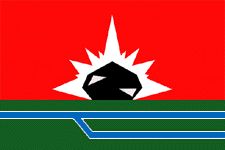
\includegraphics[width=0.3\textwidth]{img/Flag_of_Mezhdurechensk_(Kemerovo_oblast).png}

Автор герба Вадим Гущин, несмотря на нарушение ряда важных законов геральдики, сумел просто и оригинально, отказавшись от традиционных для того времени шестерёнок, колб, отбойных молотков, отразить промышленную специфику, совместив её с природно-географическим положением города.

28 августа 1966 года газета «Знамя шахтёра» представила жителям Междуреченска герб: «Щит разделён на два поля: красное (вверху) — цвет труда и зелёное (нижнее) — цвет тайги. В свете вспыхнувшей искры кусок угля — главного нашего богатства. На зелёном поле — две голубых ленты — Томь и Уса. Таким образом, герб олицетворяет две главнейшие особенности города — направленность труда его жителей и природные условия».

Автор герба совершил небольшую ошибку. Дело в том, что река Уса впадает в реку Томь с её правого берега. В гербе 1966 года сходящиеся реки изображены текущими в левую геральдическую сторону (от зрителя — в правую), что не соответствовало действительности. Ошибка была исправлена, и 18 марта 1993 года был утверждён изменённый герб.
